% !TEX encoding = UTF-8
% !TEX TS-program = pdflatex
% !TEX root = ../tesi.tex
%**************************************************************
\chapter{Archittetura del sistema AWMS}
\label{cap:archittettura del sistema AWMS}
%**************************************************************

\intro{In questo capitolo verranno descritti tutte le componenti dell'architettura AWMS e le varie operazioni di comunicazione tra le varie componenti.}\\


\section{Descrizione}
Come scritto precedentemente, dietro all'applicazione mobile c'è tutta un architettura di sistema che permette la comunicazione tra la piattaforma AWMS e l'applicazione mobile con Azzurra.
 
 \begin{figure}[h]
 	\begin{center}
 		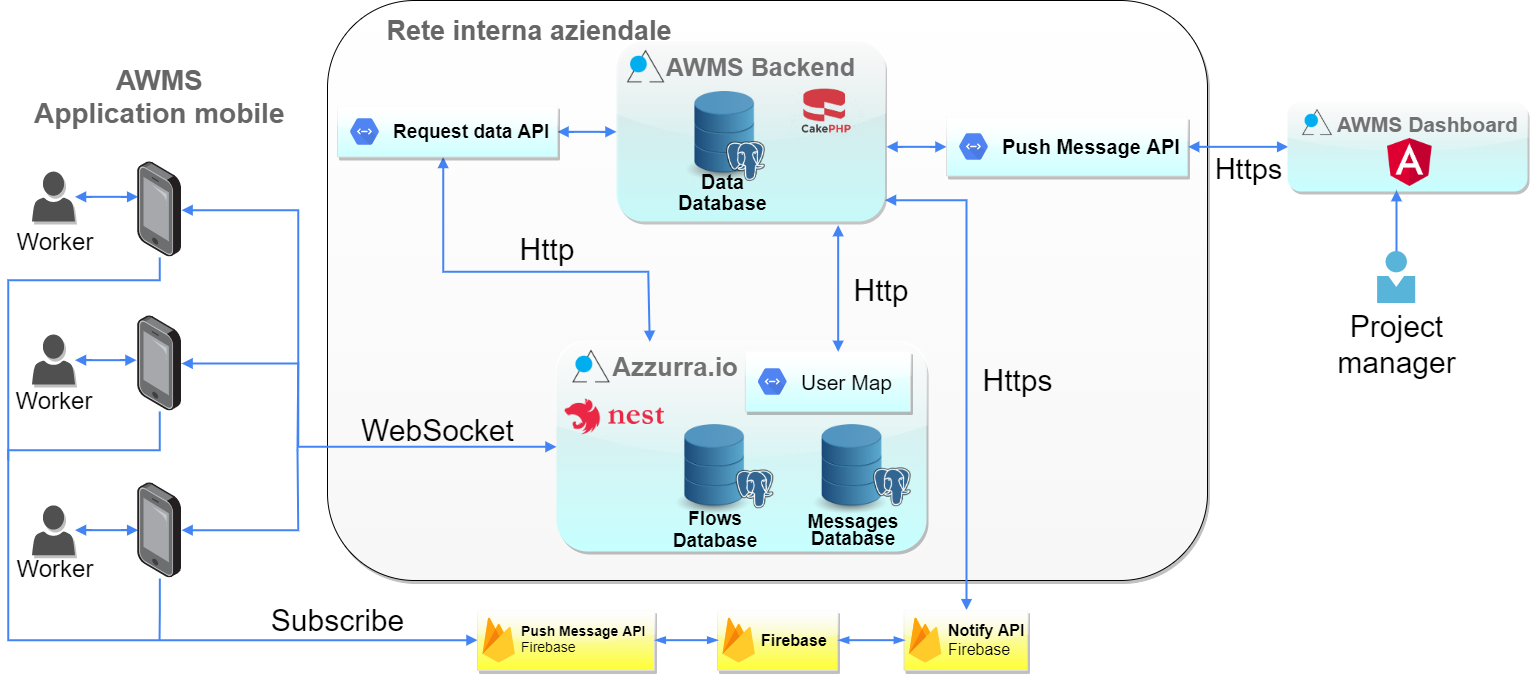
\includegraphics[scale=0.28]{AWMSDiagram.png}
 		\caption{Architettura di sistema AWMS}\label{fig:arch}
 	\end{center}
 \end{figure}
La figura precedente illustra come è composta l'architettura, dove ogni componente verrà descritta nelle successive sotto sezioni.
\begin{trivlist}
	\item \subsection{AWMS Dashboard}
	È il pannello di controllo attraverso il quale un project manager può interagire con la piattaforma AWMS per poter pianificare il lavoro da svolgere, cioè assegnare un compito alla persona più idonea. Il pannello di controllo è una applicazione web che è stata sviluppata in Angular.
	\begin{figure}[h] 
		\begin{center}
			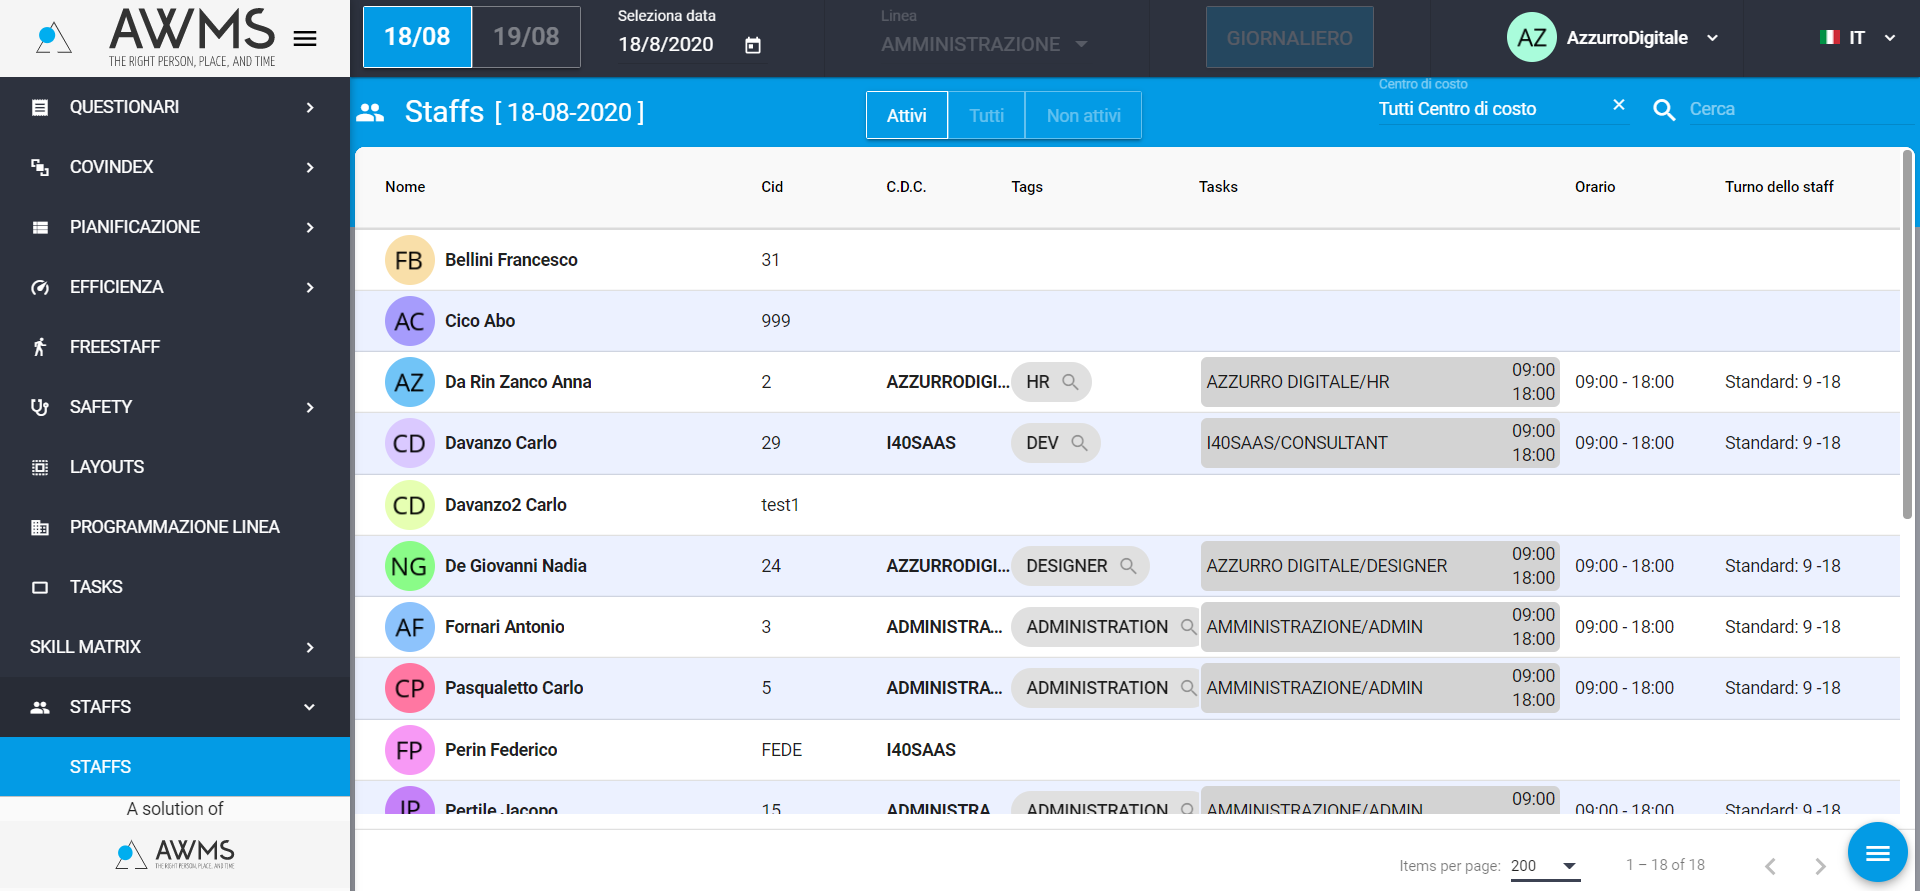
\includegraphics[scale=0.27]{dashboardAWMS.png}
			\caption{Schermata di AWMS Dashboard}
		\end{center}
	\end{figure}
	 	La dashboard per comunicare con il back-end, utilizza delle \gls{api}\ap{g} che il back-end espone, quindi per una ragione di sicurezza, back-end e l'applicazione web cioè il front-end, comunicano attraverso \gls{api}\ap{2} con in più l'utilizzo del protocollo di comunicazione HTTPS che cripta la comunicazione. Nella Figura ~\ref{fig:arch} viene mostrato il caso in cui il front-end utilizza \gls{api}\ap{3} per l'invio di notifiche push, questo perché è previsto che una volta il team leader sceglie il lavoratore più idoneo per un certo lavoro, il lavoratore deve essere avvisato, cosi sarà compito del front-end avvisare il back-end che c'è stata una nuova assegnazione e che questa assegnazione deve essere comunicata al diretto interessato attraverso un notifica sull'applicazione mobile con all'interno Azzurra.
	\item \subsection{AWMS backend}
	Come dice il suo nome, AWMS backend rappresenta il backend del sistema. AWMS backend è sviluppato usando lo strumento CakePHP, un framework per lo sviluppo di applicazioni web scritto in PHP. Al suo interno risiede il database che contiene tutte le informazioni sui lavoratori e tra questi quindi, i dati da mostrare nei messaggi di Azzurra come ad esempio il piano di lavoro che ha il lavoratore in uno specifico giorno, qualora ne venga fatta richiesta. Il database utilizza come DBMS PostgreSQL. \\
	Come detto al punto precedente, per comunicare con il backend, esso espone delle \gls{api}\ap{4} per la comunicazione infatti, esiste un \gls{api}\ap{5} per l'invio di notifiche push ma esiste anche un \gls{api}\ap{6}, utilizzata da Azzurra.io, per la richiesta di informazioni sul lavoratore necessarie per completare il flusso di conversazione. Quindi questa \gls{api}\ap{6} permetterà di richiedere dati al backend che li andrà a cercare nel suo database interno che se l'interrogazione al database da esito positivo, ritornerà le informazioni richieste a Azzurra.io. Il backend si trova all'interno della rete interna dell'azienda che ha acquistato la soluzione di AzzurroDigitale, anche Azzurra.io è all'interno della rete, perciò tra queste due componenti avviene attraverso il protocollo di comunicazione HTTP. Il backend ha la possibilità di comunicare direttamente con Azzurra.io quando deve inviare una notifica push e ha necessità di sapere quali utenti sono attivi, cioè hanno una connessione aperta con Azzurra.io. Per gli utenti invece che non hanno una connessione aperte con Azzurra.io e quindi non sono attivi l'invio della notifica verrà fatto utilizzando i servizi offerti da Firebase, la cui comunicazione tra backend e Firebase avviene tramite HTTPS perché Firebase è un servizio esterno.\\
	La gestione l'invio delle notifiche push verrà comunque tratta in modo più dettagliato più avanti nel seguente capitolo.
	\item \subsection{Azzurra.io}
	Azzurra.io è una componente strategica per il funzionamento del bot Azzurra. Azzurra.io è sviluppata attraverso il framework NestJS. Al suo interno ha due database con DBMS PostgreSQL. Il primo database contiene i flussi di conversazione i quali indicano al bot che sequenza di passi deve fare durante la conversazione con l'utente umano, la loro struttura verrà spiegata in modo dettagliato al capitolo successivo. Il secondo database permette di memorizzare i messaggi fatti tra il bot Azzurra e l'utente umano. La scelta di adottare quest'ultimo database è dettata dalle seguenti motivazioni:
	\begin{itemize}
		\item Per mantenere lo stato della conversazione cioè, se l'utente decide di non andare avanti con la conversazione e di continuarla in un secondo momento, grazie a questo database, in cui viene salvato lo stato della conversazione, potrà continuare la conversazione da dove l'aveva lasciata;
		\item Per una migliore user experience si è scelto, nel caso in cui ci siano state delle conversazioni in precedenza, di mostrare i messaggi delle conversazioni precedenti, cosi che se l'utente ha bisogno di un’informazione  che ha già chiesto precedentemente ma che si è dimenticato, basta che controlli i messaggi presenti nella chat senza dover richiedere ad Azzurra l'informazione dimenticata.
	\end{itemize}
	La connessione tra l'applicazione mobile e Azzurra.io è possibile grazie ai websocket che permettono di aprire una connessione tra i due e di mantenere sempre aggiornati i dati ad esempio la struttura dei flussi di conversazione, qualora venissero aggiornati. Per tenere traccia dei utenti connessi con Azzurra.io tramite l'applicazione mobile, viene utilizzata la mappa chiave-valore, interna ad Azzurra.io denominata User Map, la quale servirà a rispondere alle richieste del backend quando avrà bisogno della lista di utenti attivi per l'invio della notifica push. Come detto all'inizio del punto Azzurro.io è un componente strategico per principalmente due motivi.
	\begin{itemize}
		\item Quando si vuole aggiungere un nuovo flusso conversazionale o modificare un flusso già esistente, se non esistesse Azzurra.io, questi sarebbero salvati nell'applicazione che ne comporterebbe l'aggiornamento dell'applicazione mobile e quindi effettuare una nuova pubblicazione nell'Play Store per i dispositivi Android e nel Apple Store per i dispositivi iOS ad ogni aggiunta o modifica dei flussi. Grazie all'esistenza di Azzurra.io ciò viene evitato perché esiste il database dedicato per la memorizzazione dei flussi conversazionali che se c'è da aggiungere un nuovo flusso basta semplicemente inserirlo all'interno del database, analogamente per la modifica di un flusso. Inoltre, grazie alla connessione tramite websocket qualunque modifica o aggiunta viene subito recepita dell'applicazione mobile;
		\item Per evitare che vengano fatte un numero elevato di richieste al backend si è deciso di distribuire le informazioni in diverse componenti della rete, infatti il bot per sapere che flusso conversazionale deve seguire per genere i messaggi per la conversazione con l'utente umano, chiede a Azzurra.io e non al backend. Il backend però verrà contattato quando il bot Azzurra ha bisogno di dati sul lavoratore da mostrare, questa richiesta però sarà fatta inizialmente a Azzurra.io che si prenderà carico di richiedere le informazioni al backend e di ritornarle all'applicazione. Quindi il backend sarà contattato solo dalla dashboard e da Azzurra.io per il caso descritto precedentemente per il processo di autenticazione dell'utente, diminuendo il carico sul backend.
	\end{itemize}
	
	\item\subsection{Applicazione mobile}
	L'ultimo componente dell'architettura e l'applicazione mobile. Essa è sviluppata attraverso il framework Angular2+ e Ionic e al suo interno risiede il bot Azzurra. Oltre al bot Azzurra esisto altre due sezioni, la sezione questionario e la sezione profilo. 
	
	\begin{figure}[h]
		\centering
		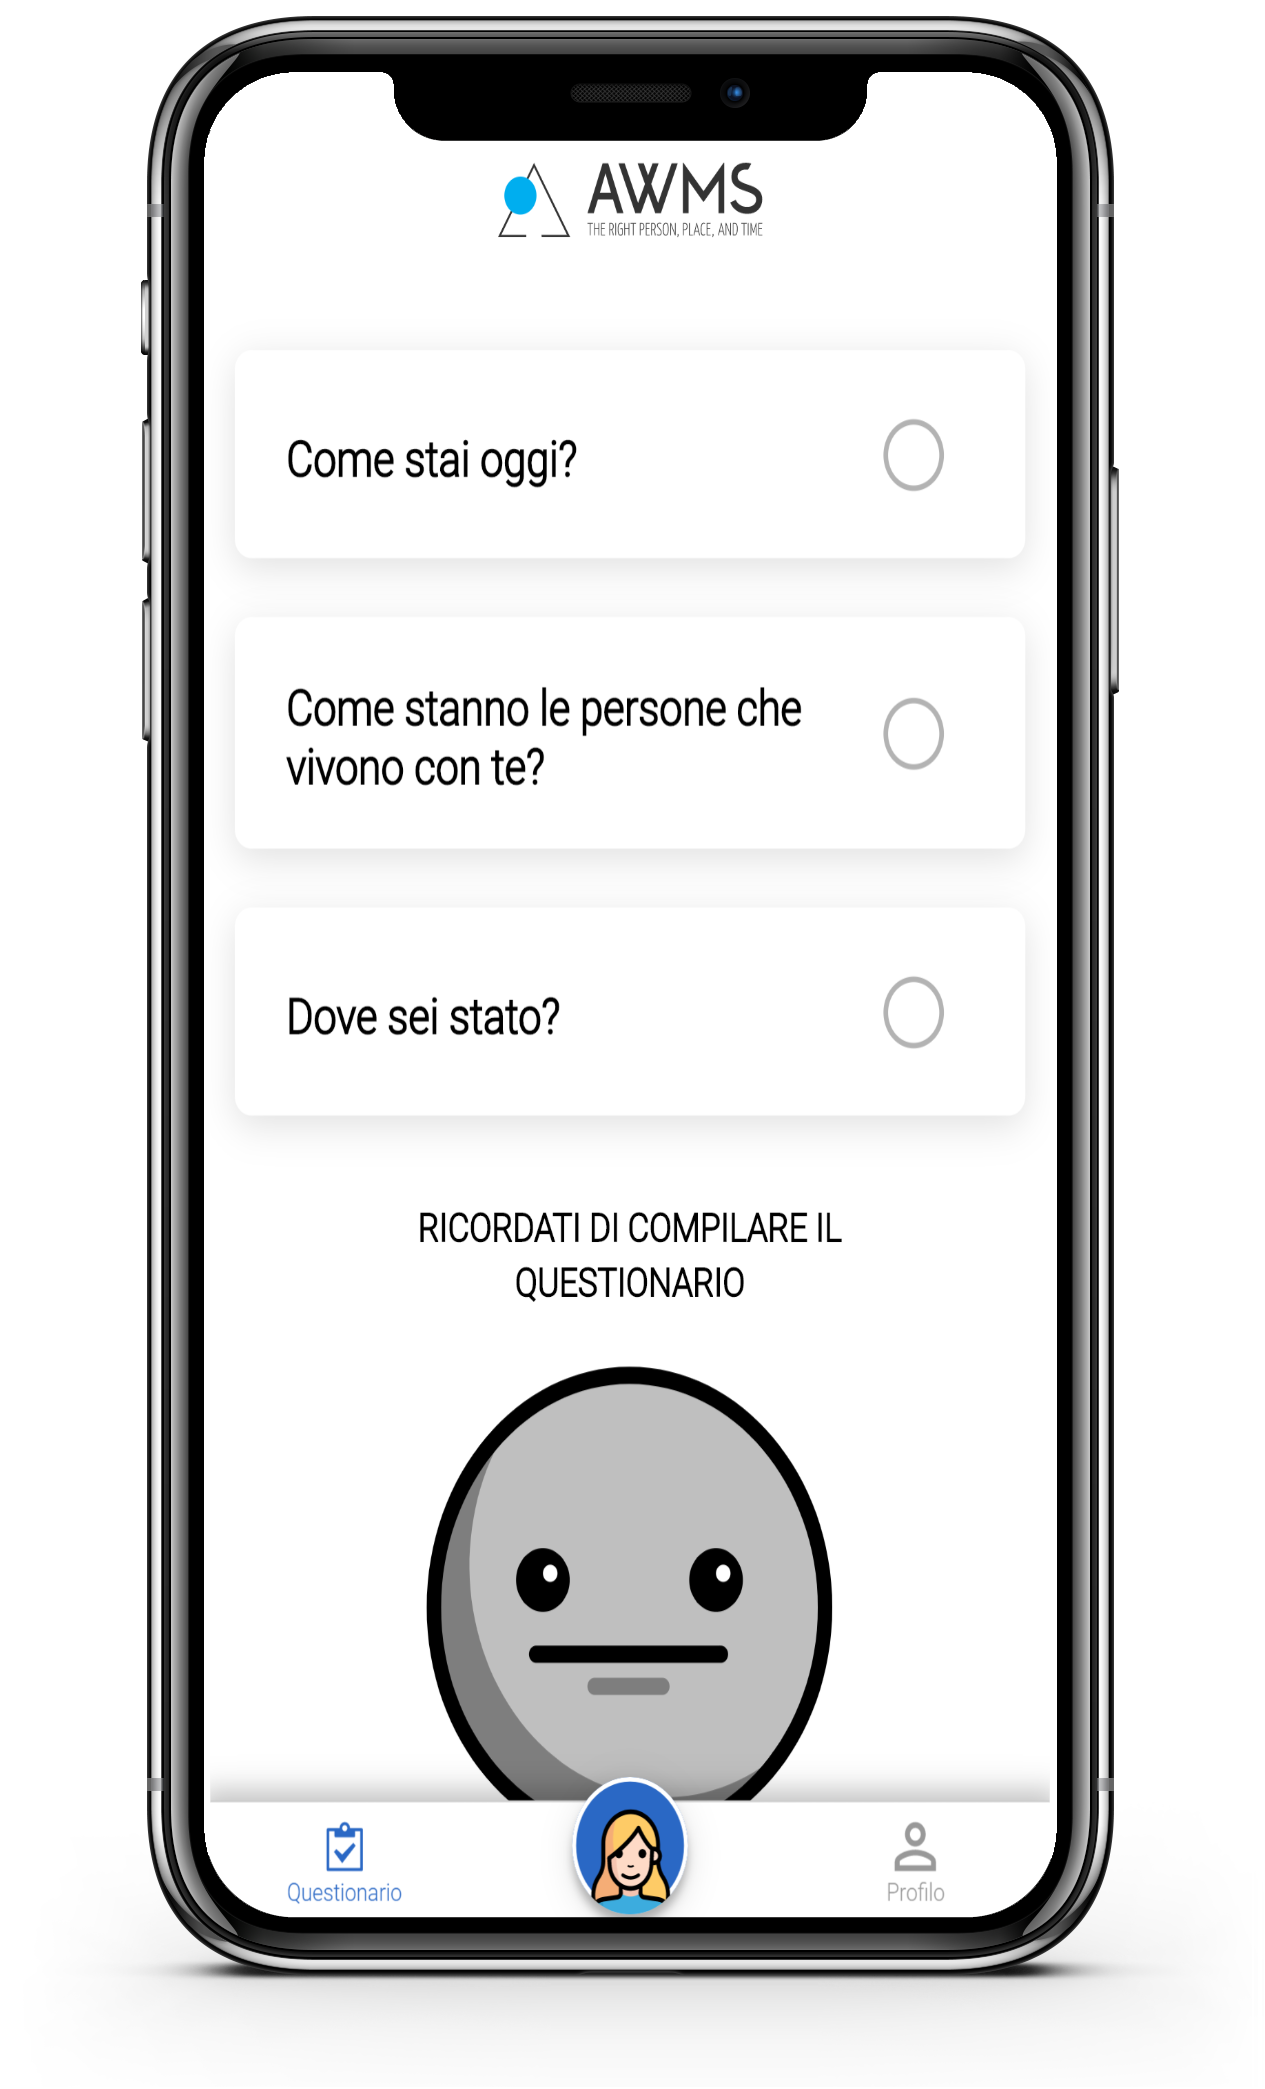
\includegraphics[scale=0.13]{queGrey.png}\hfill
		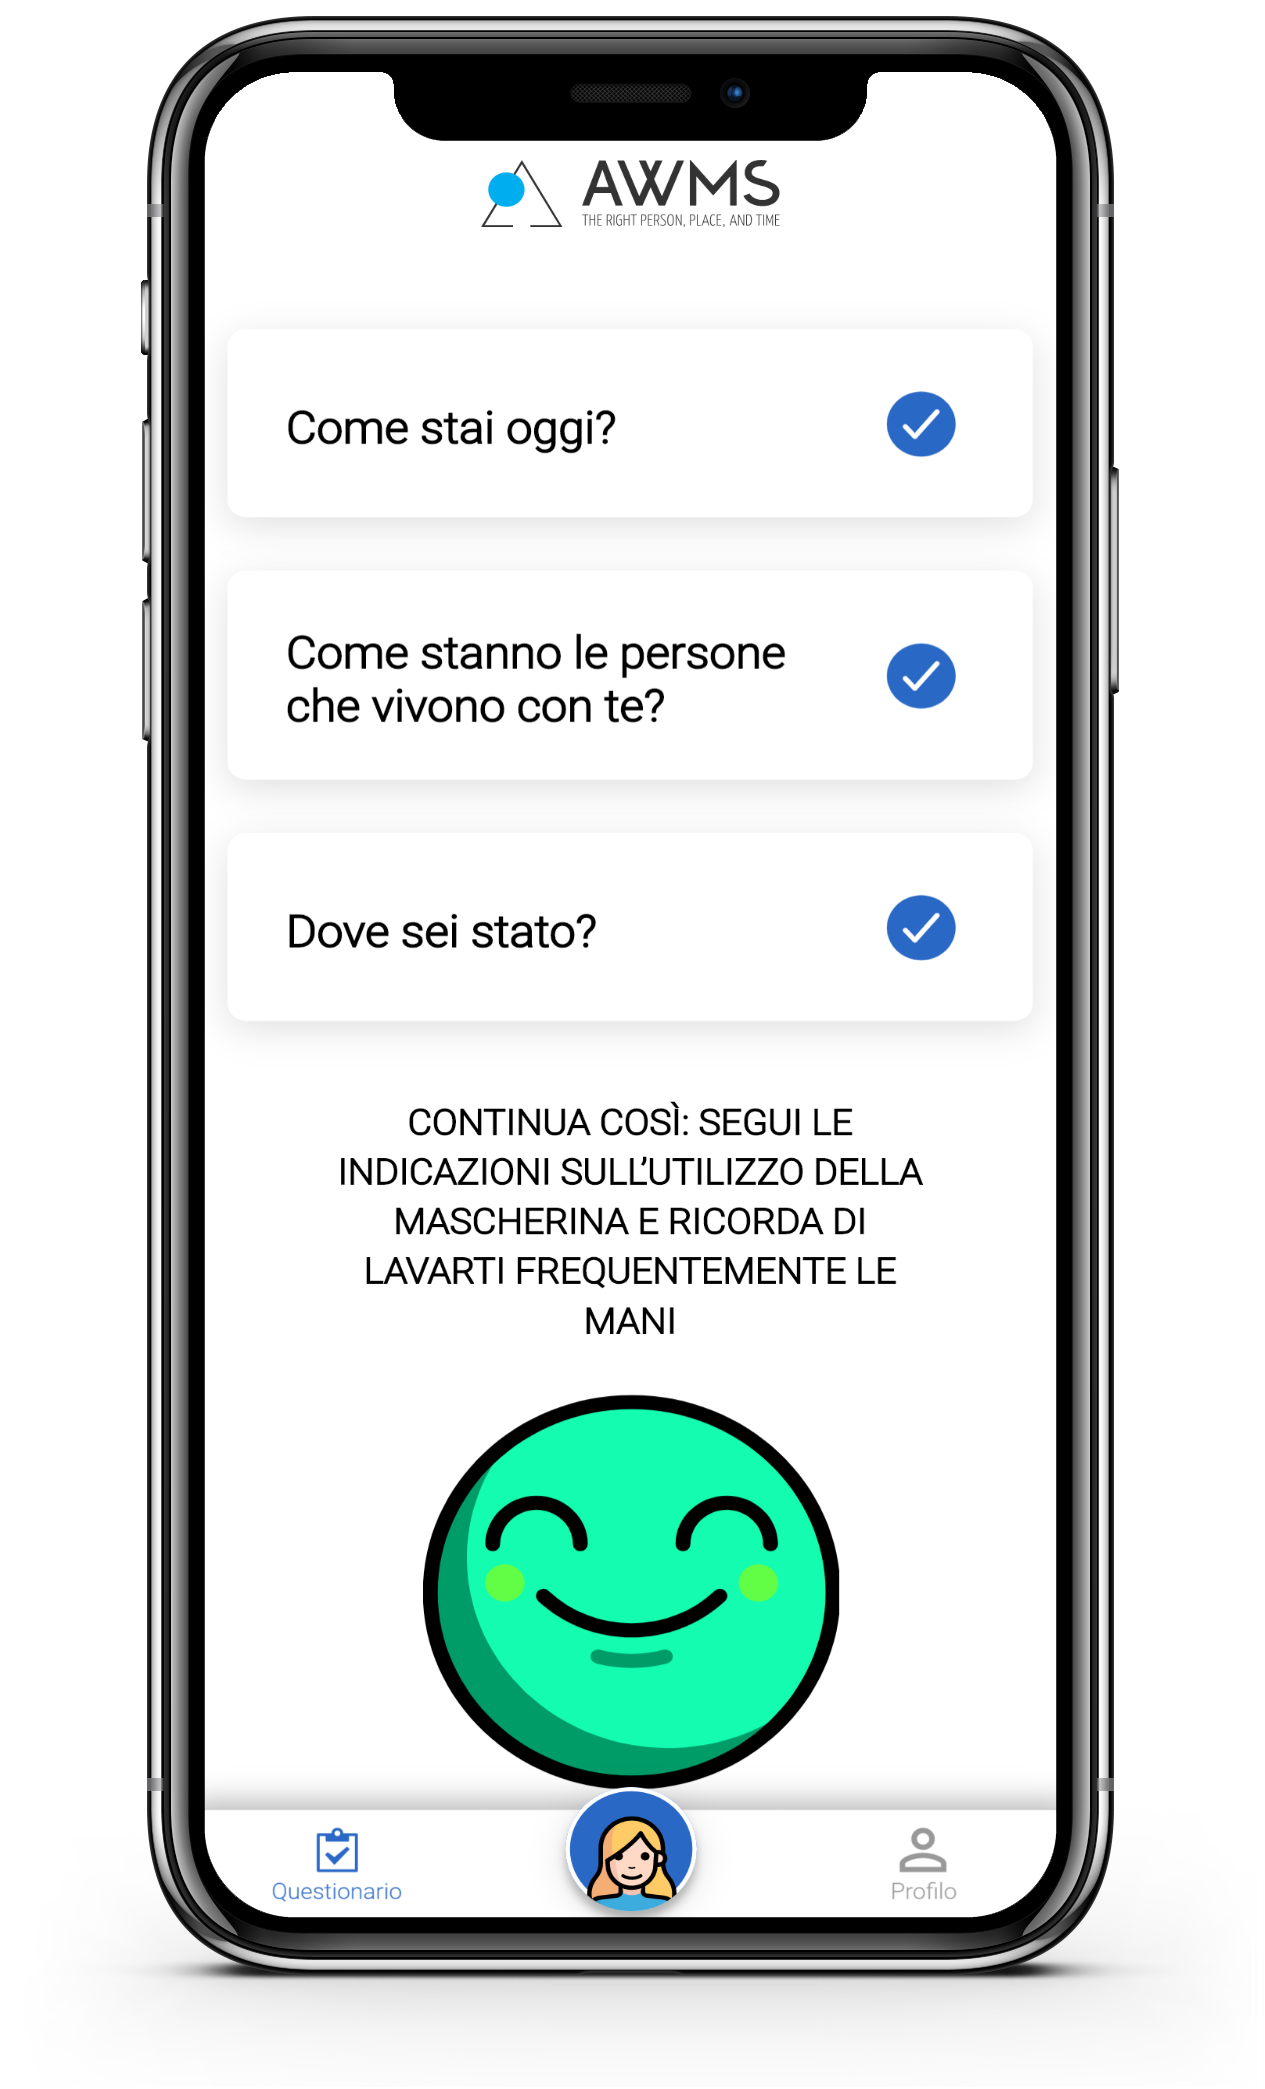
\includegraphics[scale=0.13]{queGreen.png}\hfill
		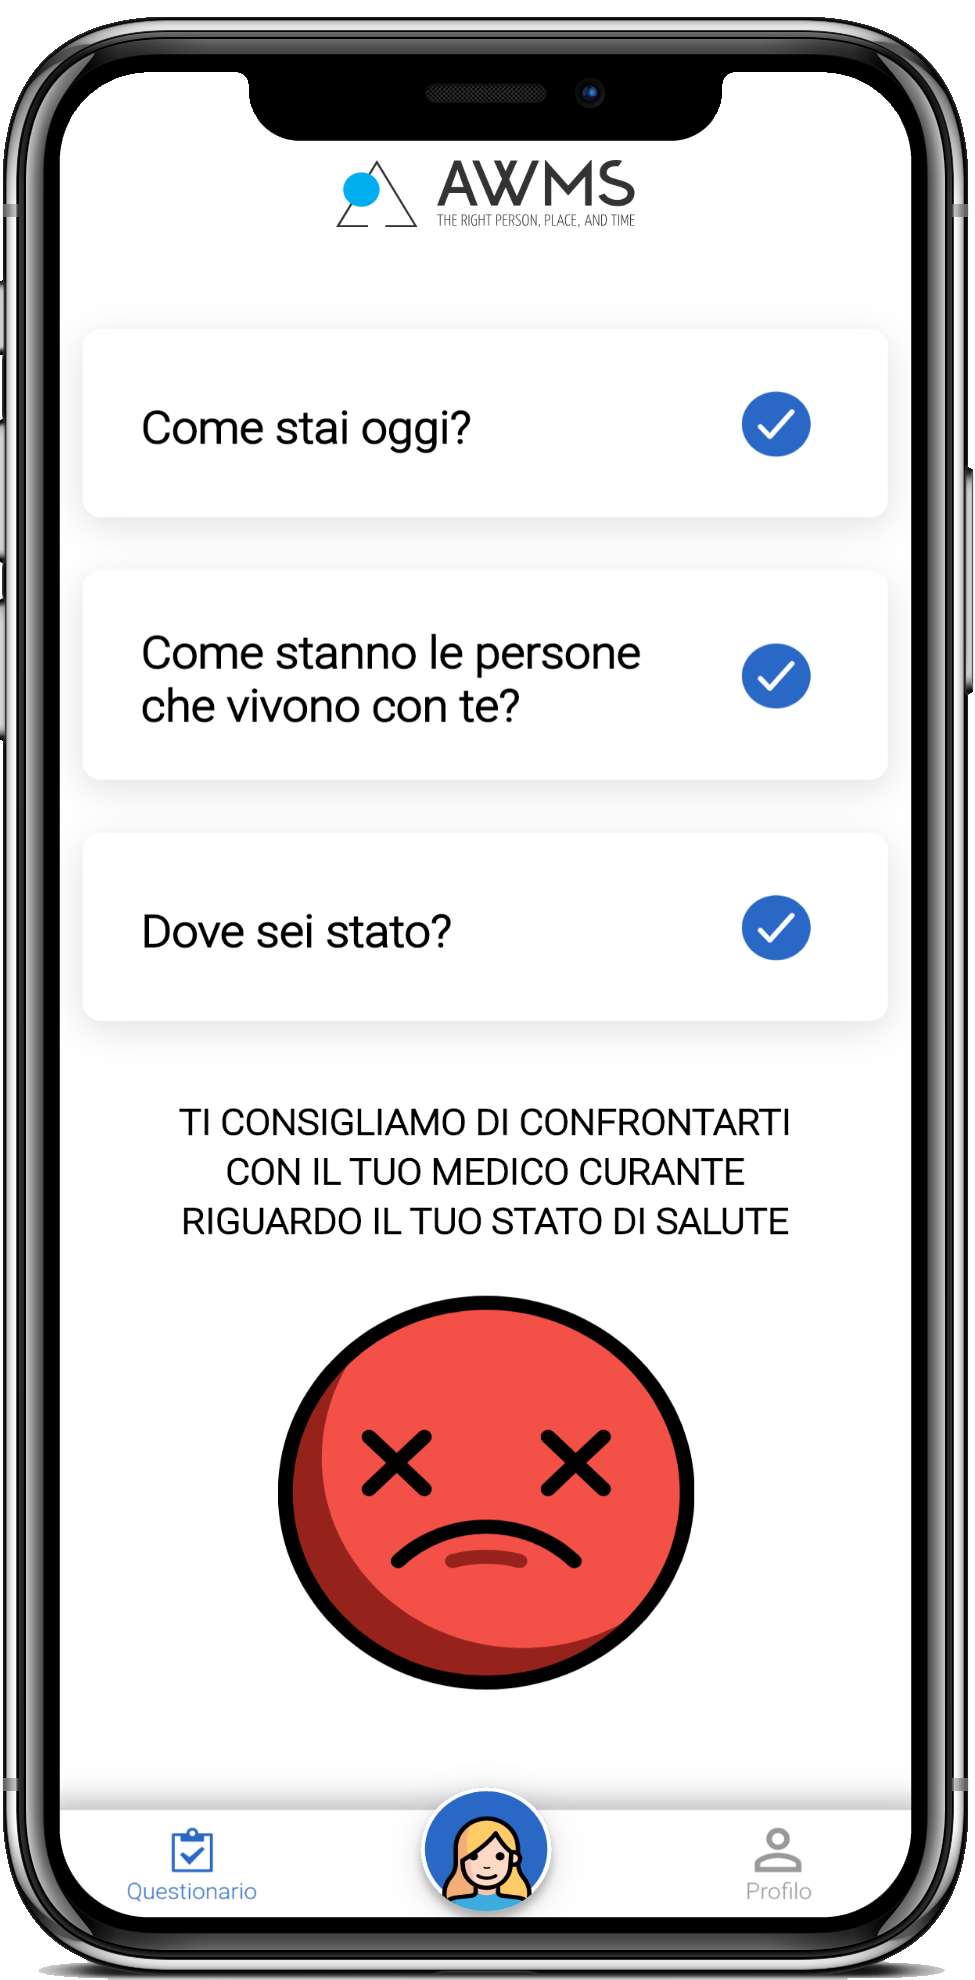
\includegraphics[scale=0.13]{queRed.png}
		\caption{Sezione Questionario}\label{fig:que}
	\end{figure}
	
	La figura ~\ref{fig:que} mostra la sezione Questionario nei sue 3 possibili stati. In questa sezione viene richiesto di compilare quotidianamente un questionario in cui vengono poste domande sulla propria salute che, dai dati raccolti per ogni lavoratore l'applicazione cerca di capire se all'interno dell'azienda ci sia pericolo di contagio del virus COVID-19. Nel caso in cui non si è ancora compilato il questionario, viene mostrata una faccina grigia come si può vedere nella prima immagine della figura ~\ref{fig:que}. Se si è compilato il questionario e secondo le risposte date si risulta essere in buona salute, allora l'applicazione mostrerà una faccina verde come si può vedere nella seconda immagine della figura ~\ref{fig:que}. Se si è compilato il questionario e secondo le risposte date si risulta essere a rischio con la propria salute, allora l'applicazione mostrerà una faccina rossa come si può vedere dalla terza immagine della figura ~\ref{fig:que}.
	\\
	\clearpage
	In questa sezione viene richiesto di compilare un questionario dove vengono richiesti se si hanno avuto dei sintomi di malattie come mostra la prima immagine della figura ~\ref{fig:queSlide}. Successivamente viene richiesto se le persone vicino a noi hanno avuto qualche sintomo di malattie come mostrato nella seconda immagine della figura ~\ref{fig:queSlide}. Viene poi richiesto in quelli luoghi si è stati come mostrato nella seconda immagine della figura ~\ref{fig:queSlide}.
	\begin{figure}[h]
		\begin{center}
			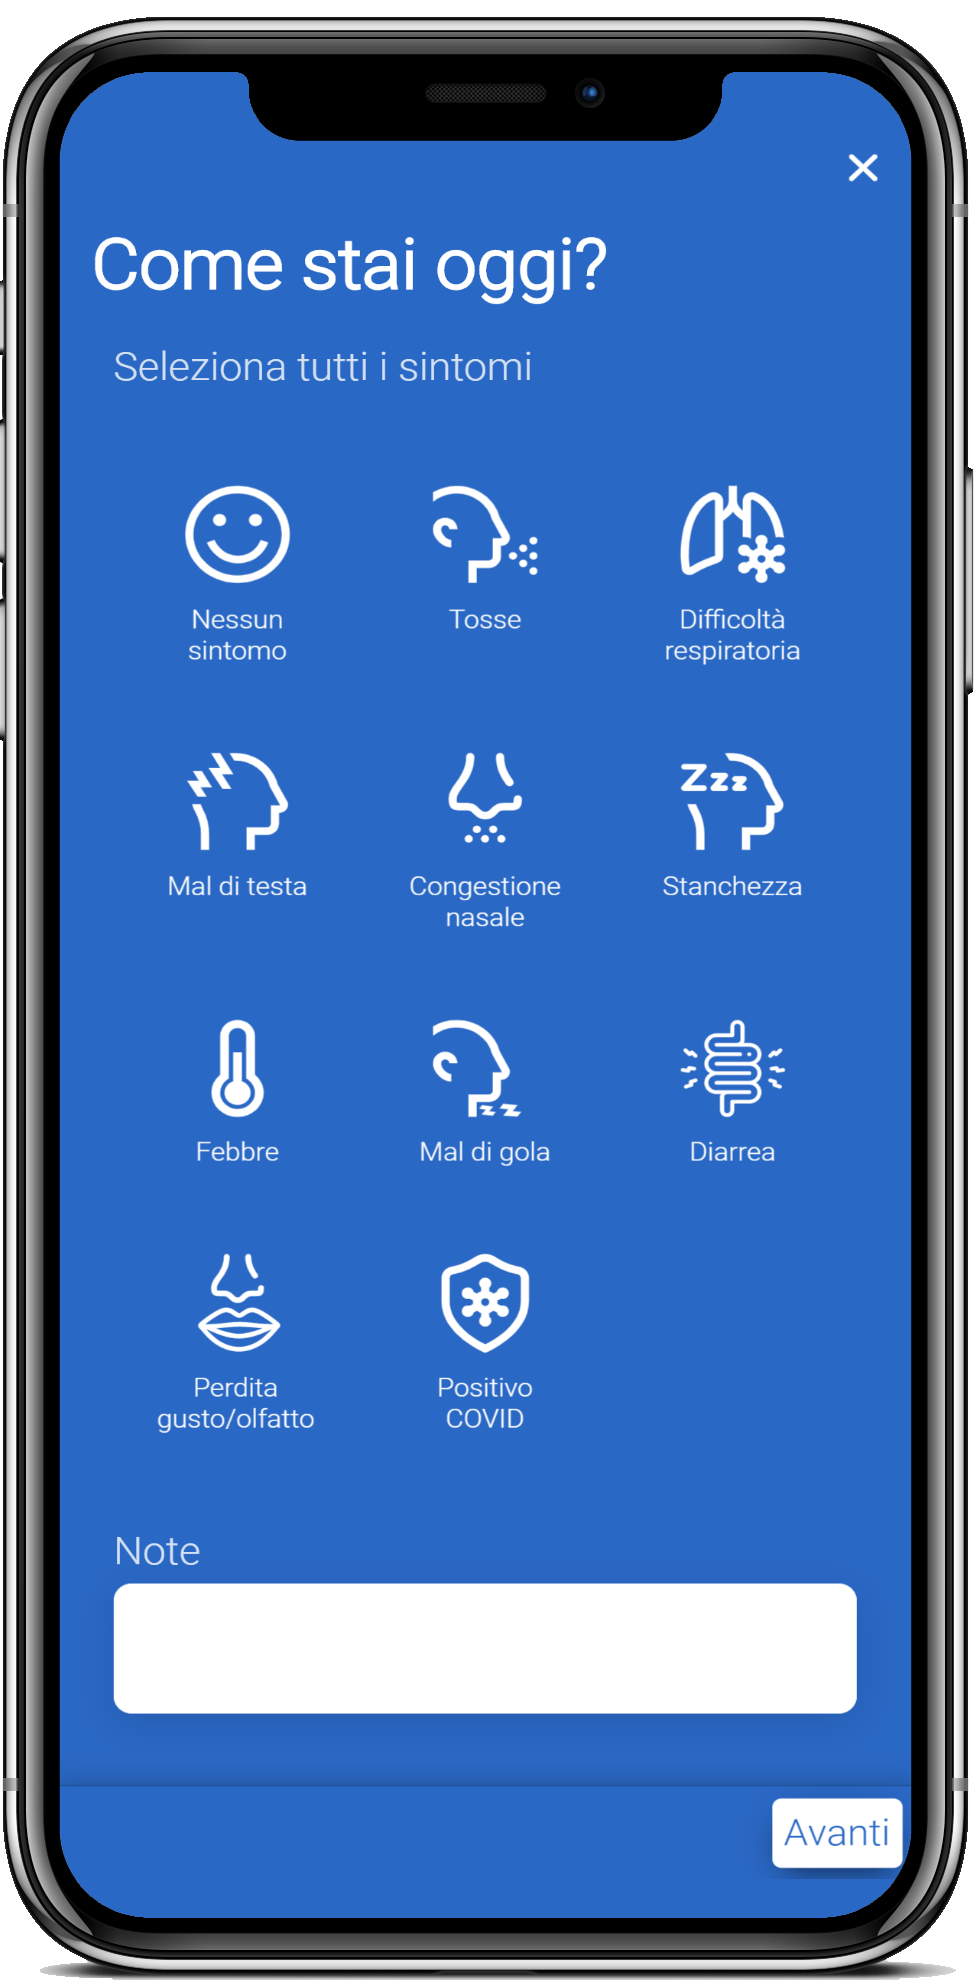
\includegraphics[scale=0.12]{que1.png}
			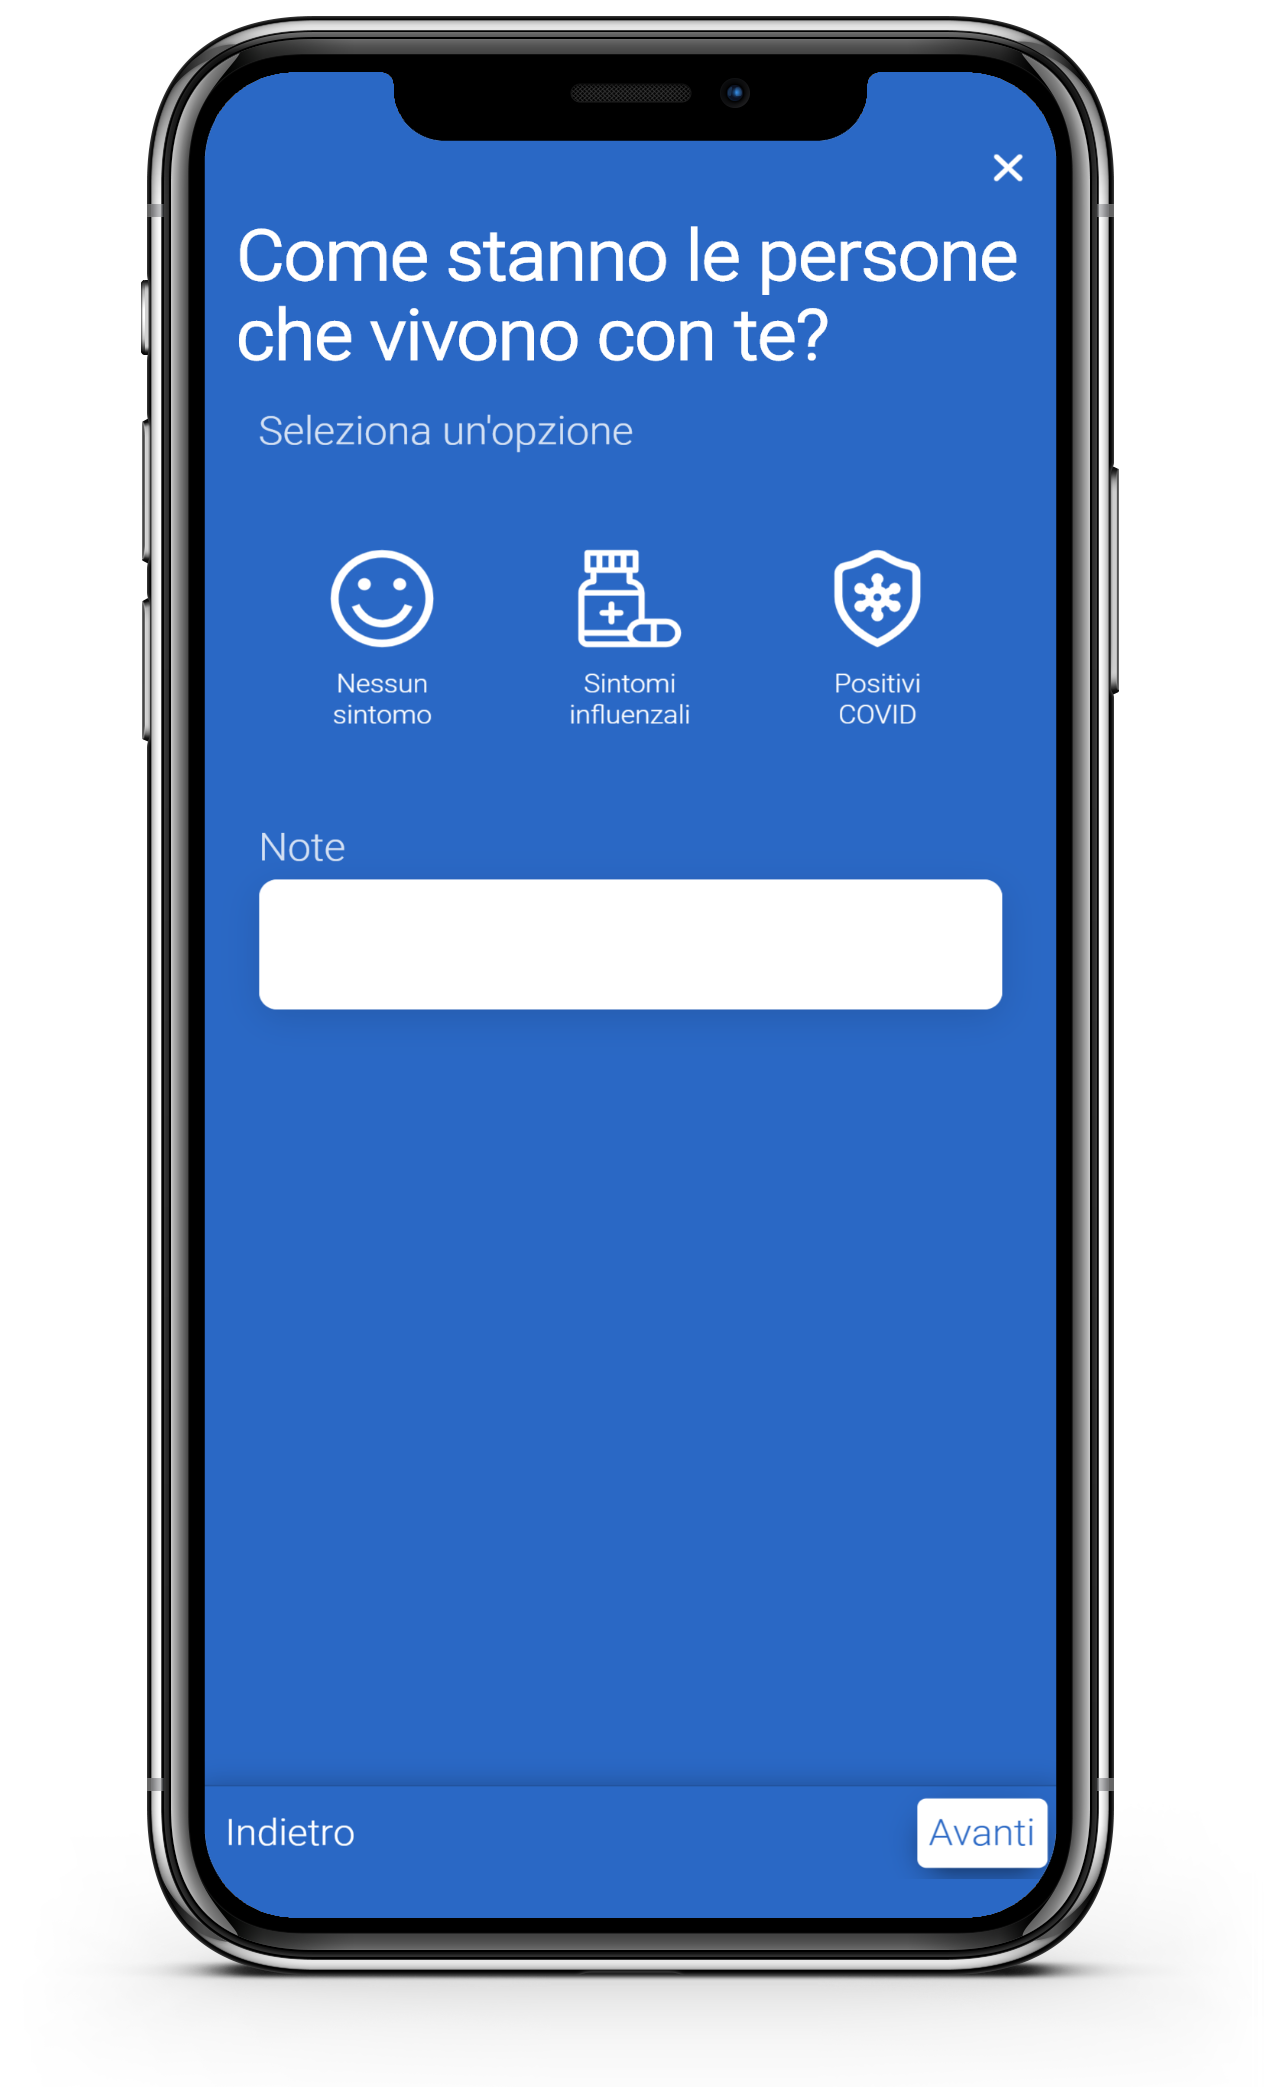
\includegraphics[scale=0.12]{que2.png}
			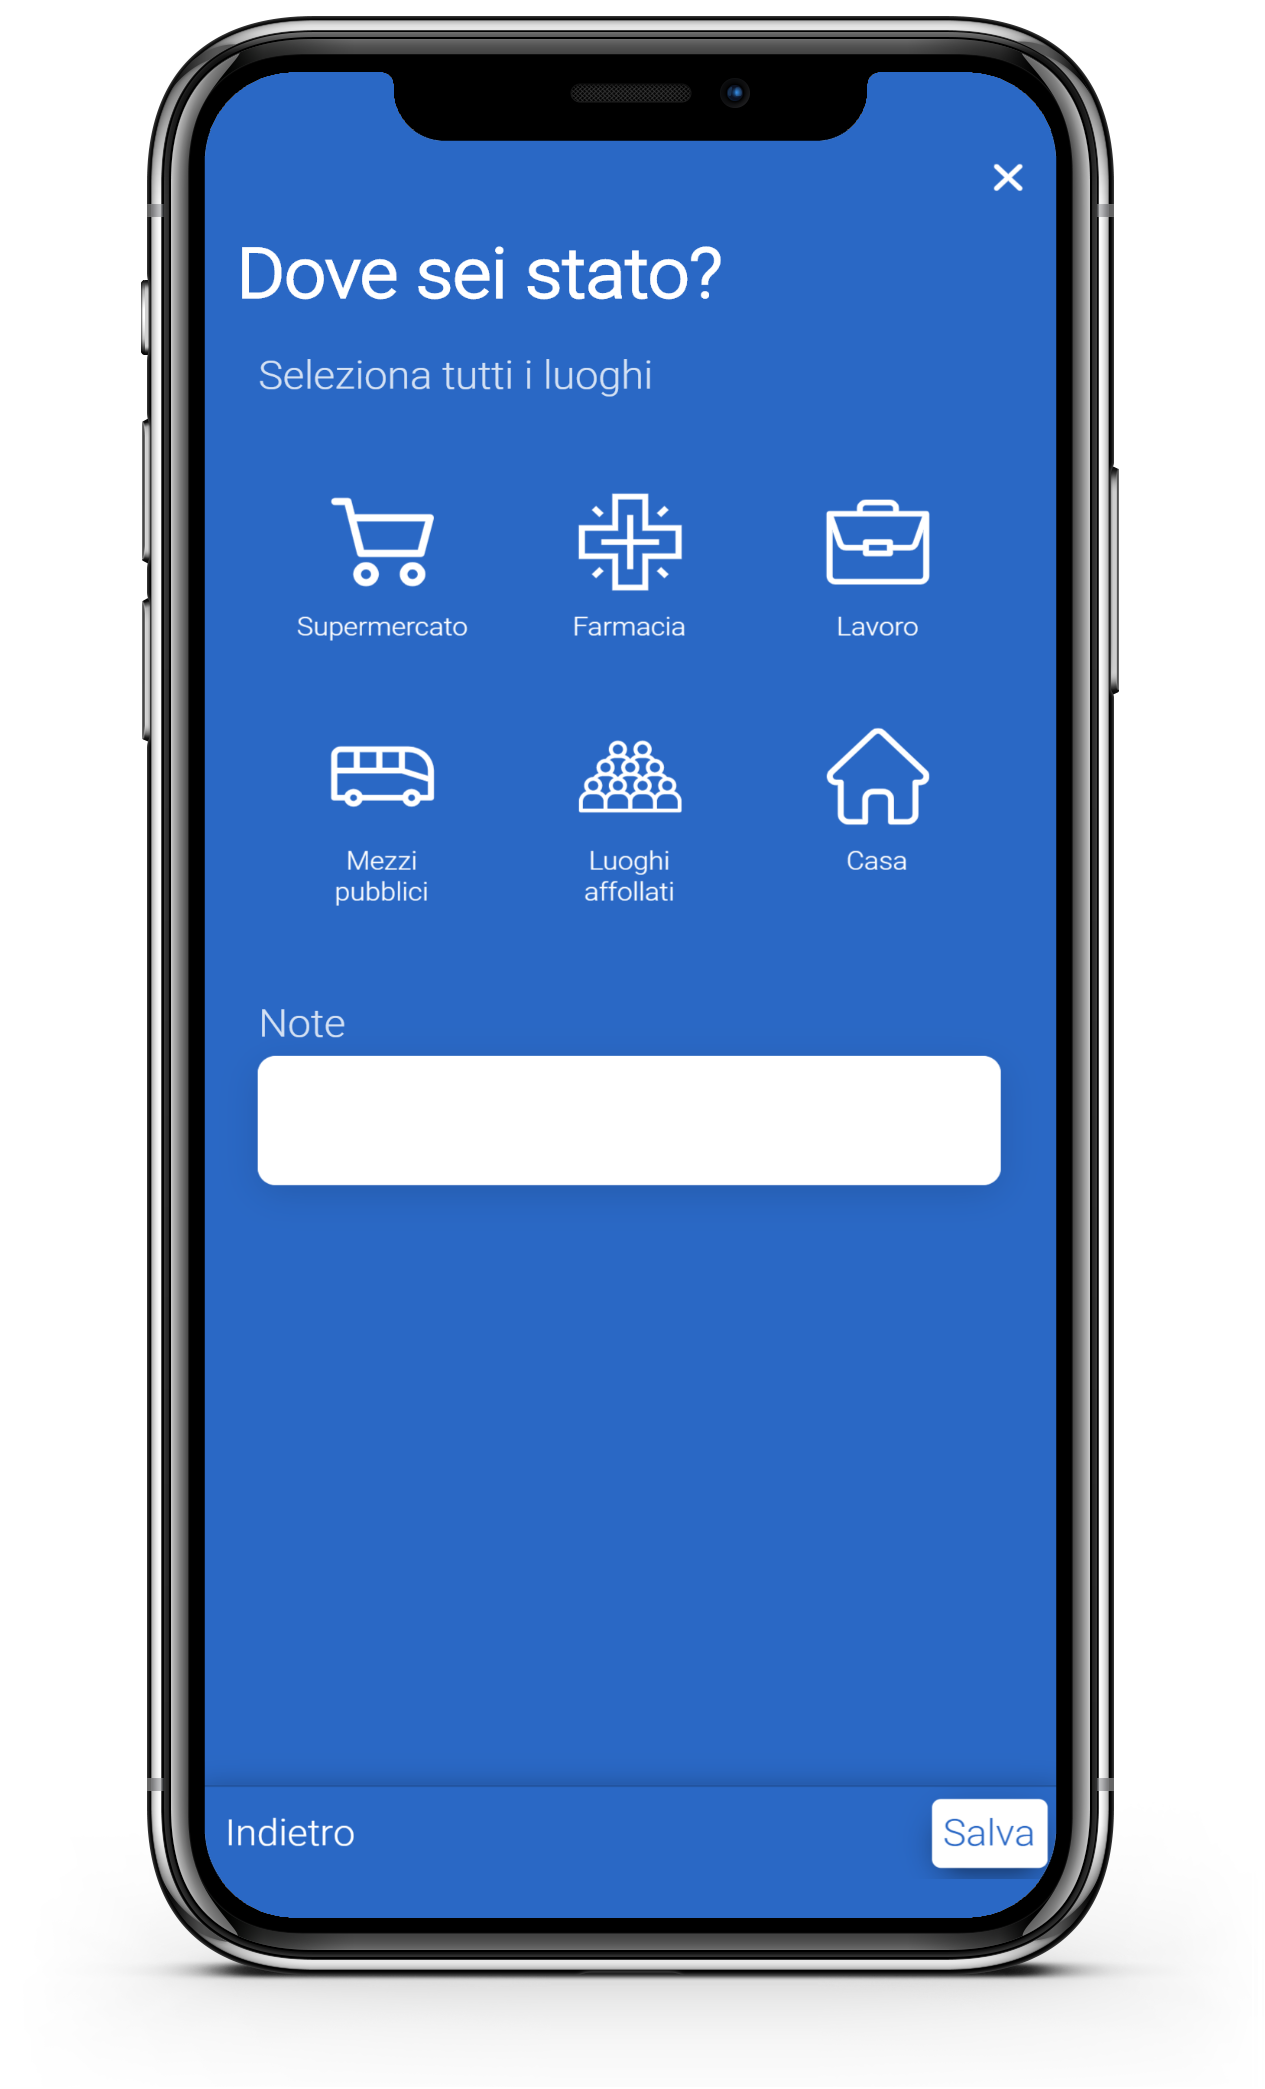
\includegraphics[scale=0.12]{que3.png}
			\caption{Schede del questionario sulla salute}\label{fig:queSlide}
		\end{center}
	\end{figure}

	Una volta terminato il questionario, l'applicazione elaborare le risposte date e mostrerà l'esito sulla nostra salute. Nel caso in cui l'esito sia positivo verrà mostrata la prima immagine della figura ~\ref{fig:quefinal} invece in caso di esito negativo verrà mostrata la seconda immagine della figura ~\ref{fig:quefinal}.
	\begin{figure}[h]
		\begin{center}
			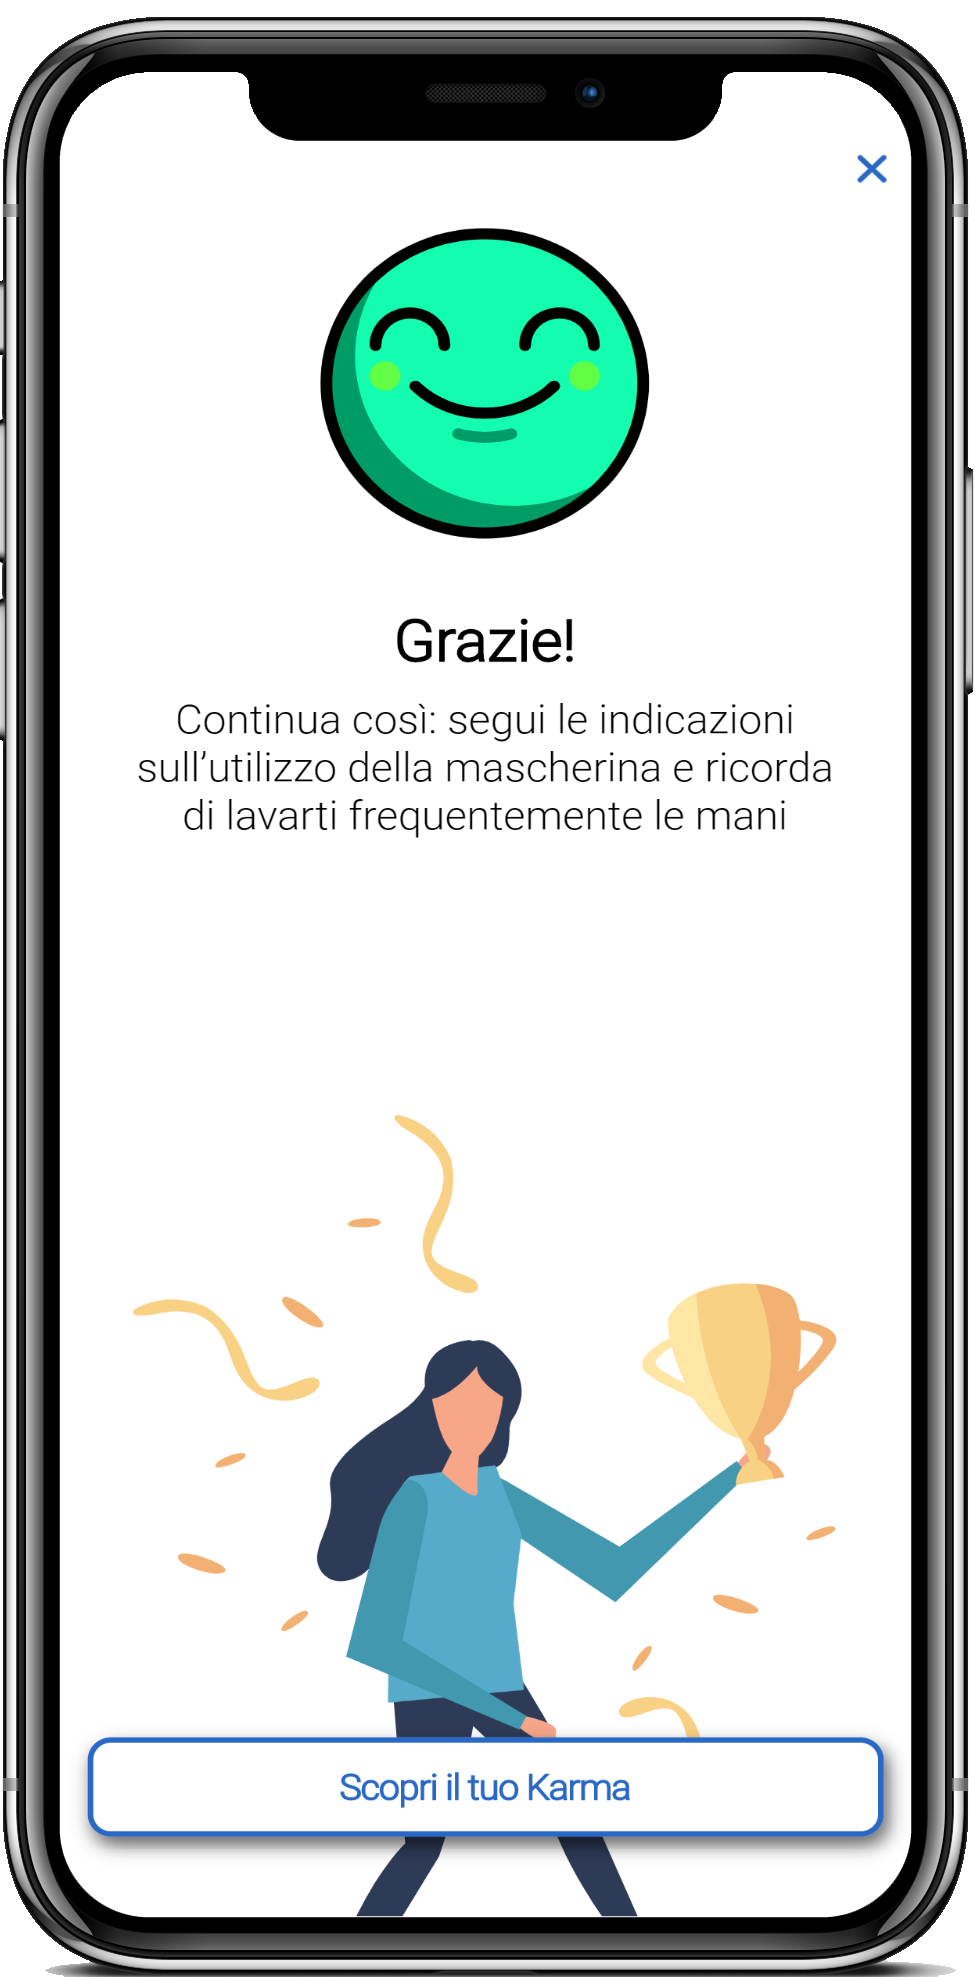
\includegraphics[scale=0.12]{finalGreen.png}
			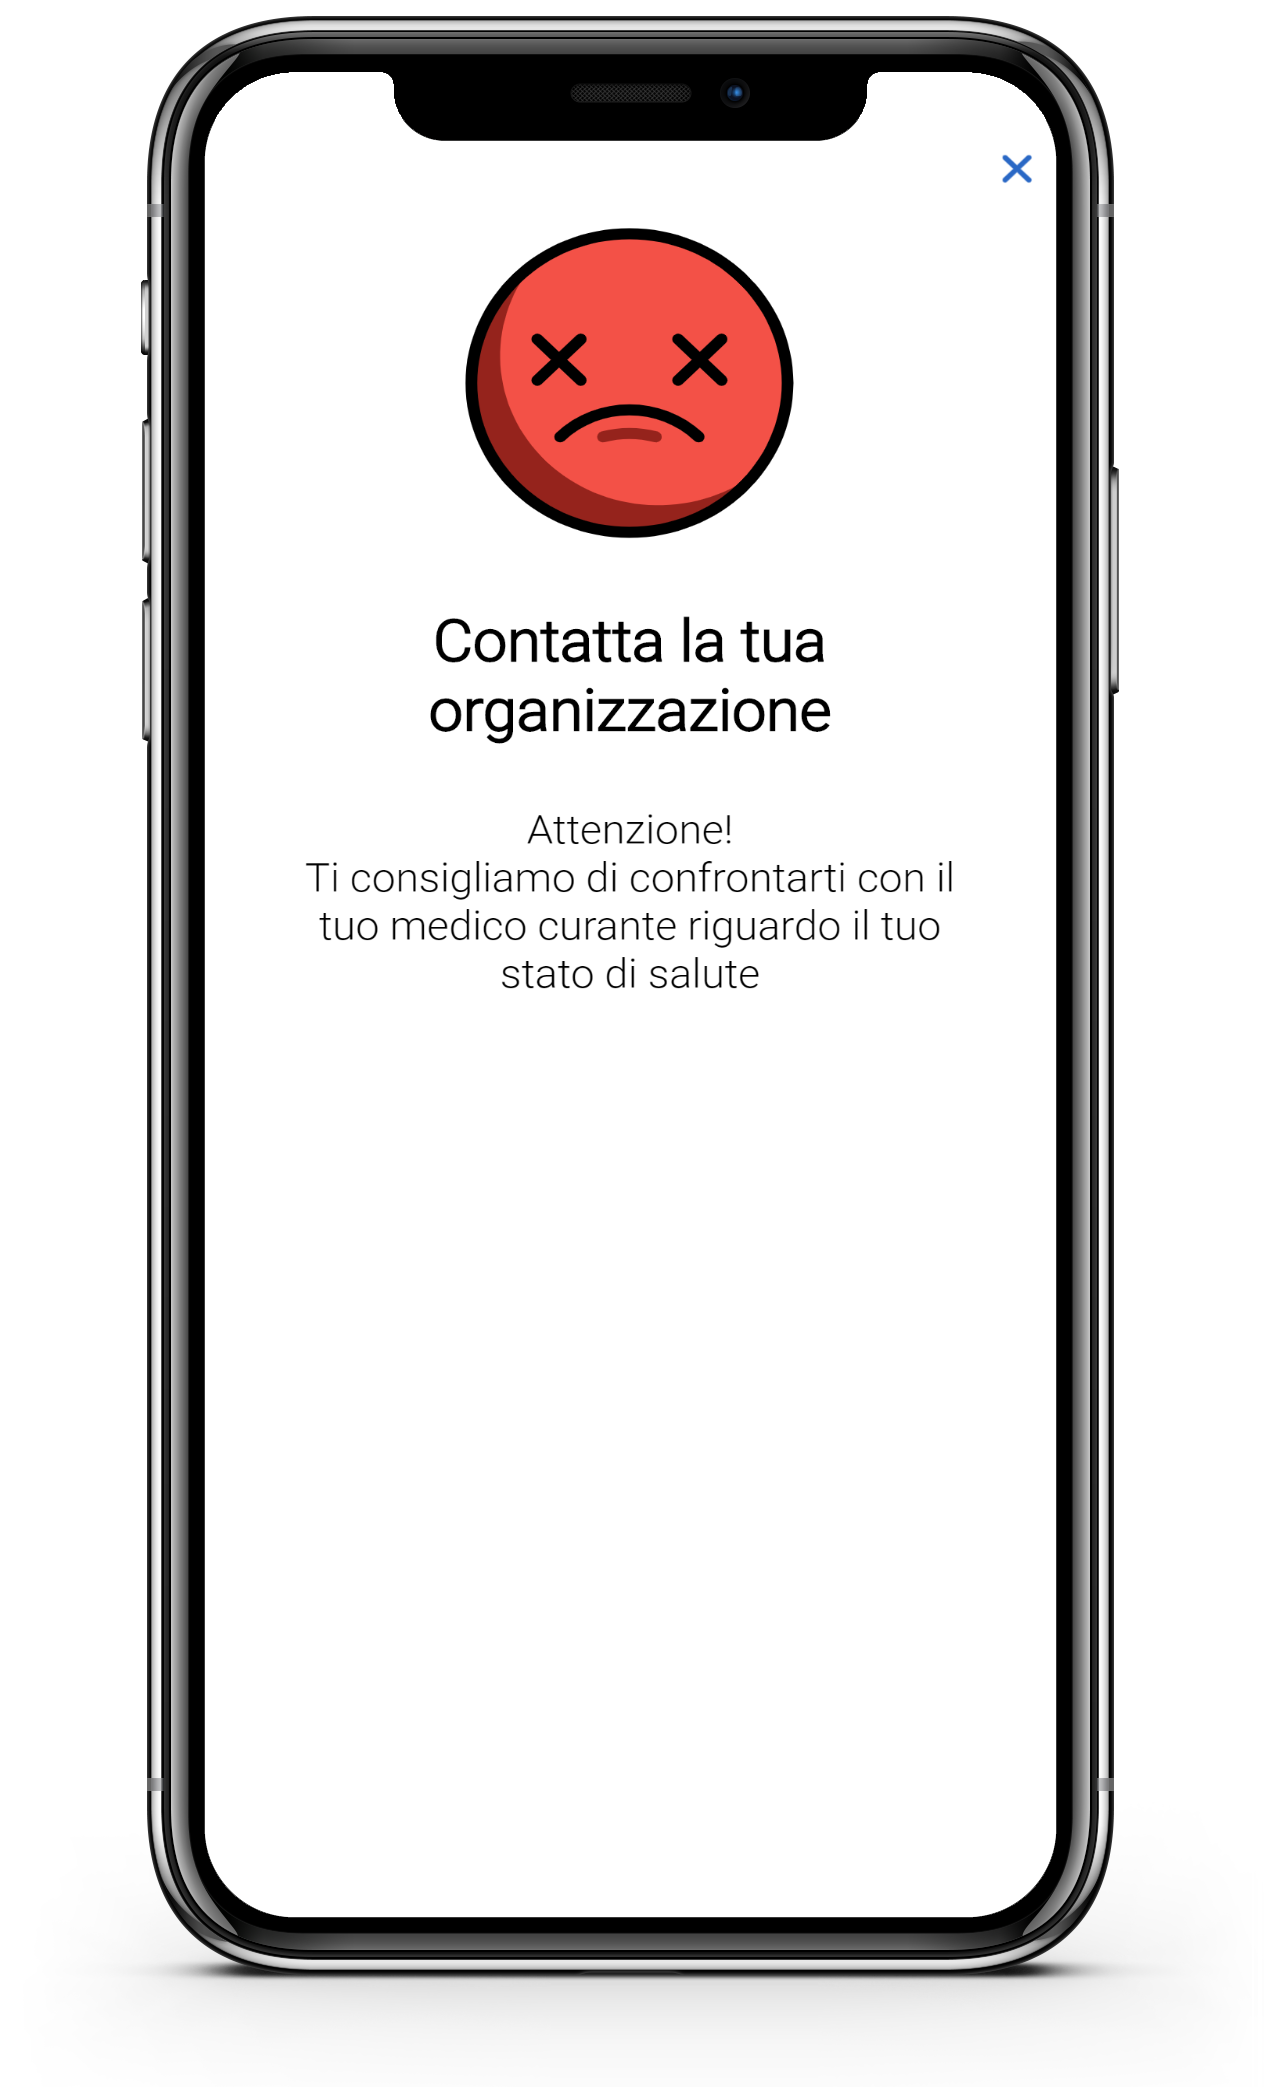
\includegraphics[scale=0.12]{finalRed.png}
			\caption{Schede dell'esito del questionario sulla salute}\label{fig:quefinal}
		\end{center}
	\end{figure}\\
	Il risultato viene poi riportato anche nella schermata della sezione Questionario.
	\\
	Nella sezione Profilo invece, vengono mostrati i Karma points che sono stati raccolti durante la compilazione del questionario, punti che al momento non danno nessun particolare beneficio ma, in futuro è previsto l'implementazione di una qualche ricompensa. Vengono mostrate le proprie informazioni personali cliccando il tasto Informazioni personali come mostrato in figura ~\ref{fig:profile}, e possibile cambiare la password d'accesso cliccando il bottone Gestione password. Cliccando il bottone Istruzione di utilizzo mostrato sempre nella figura ~\ref{fig:profile} e possibile accedere a una breve guida su come utilizzare l'applicazione. Nel bottone Normativa privacy è possibile visionare la normativa sulla tutela della privacy GDPR mentre nel bottone Titolare trattamento viene indicato da chi vengono trattati i dati inseriti.
	\begin{figure}[h]
		\begin{center}
			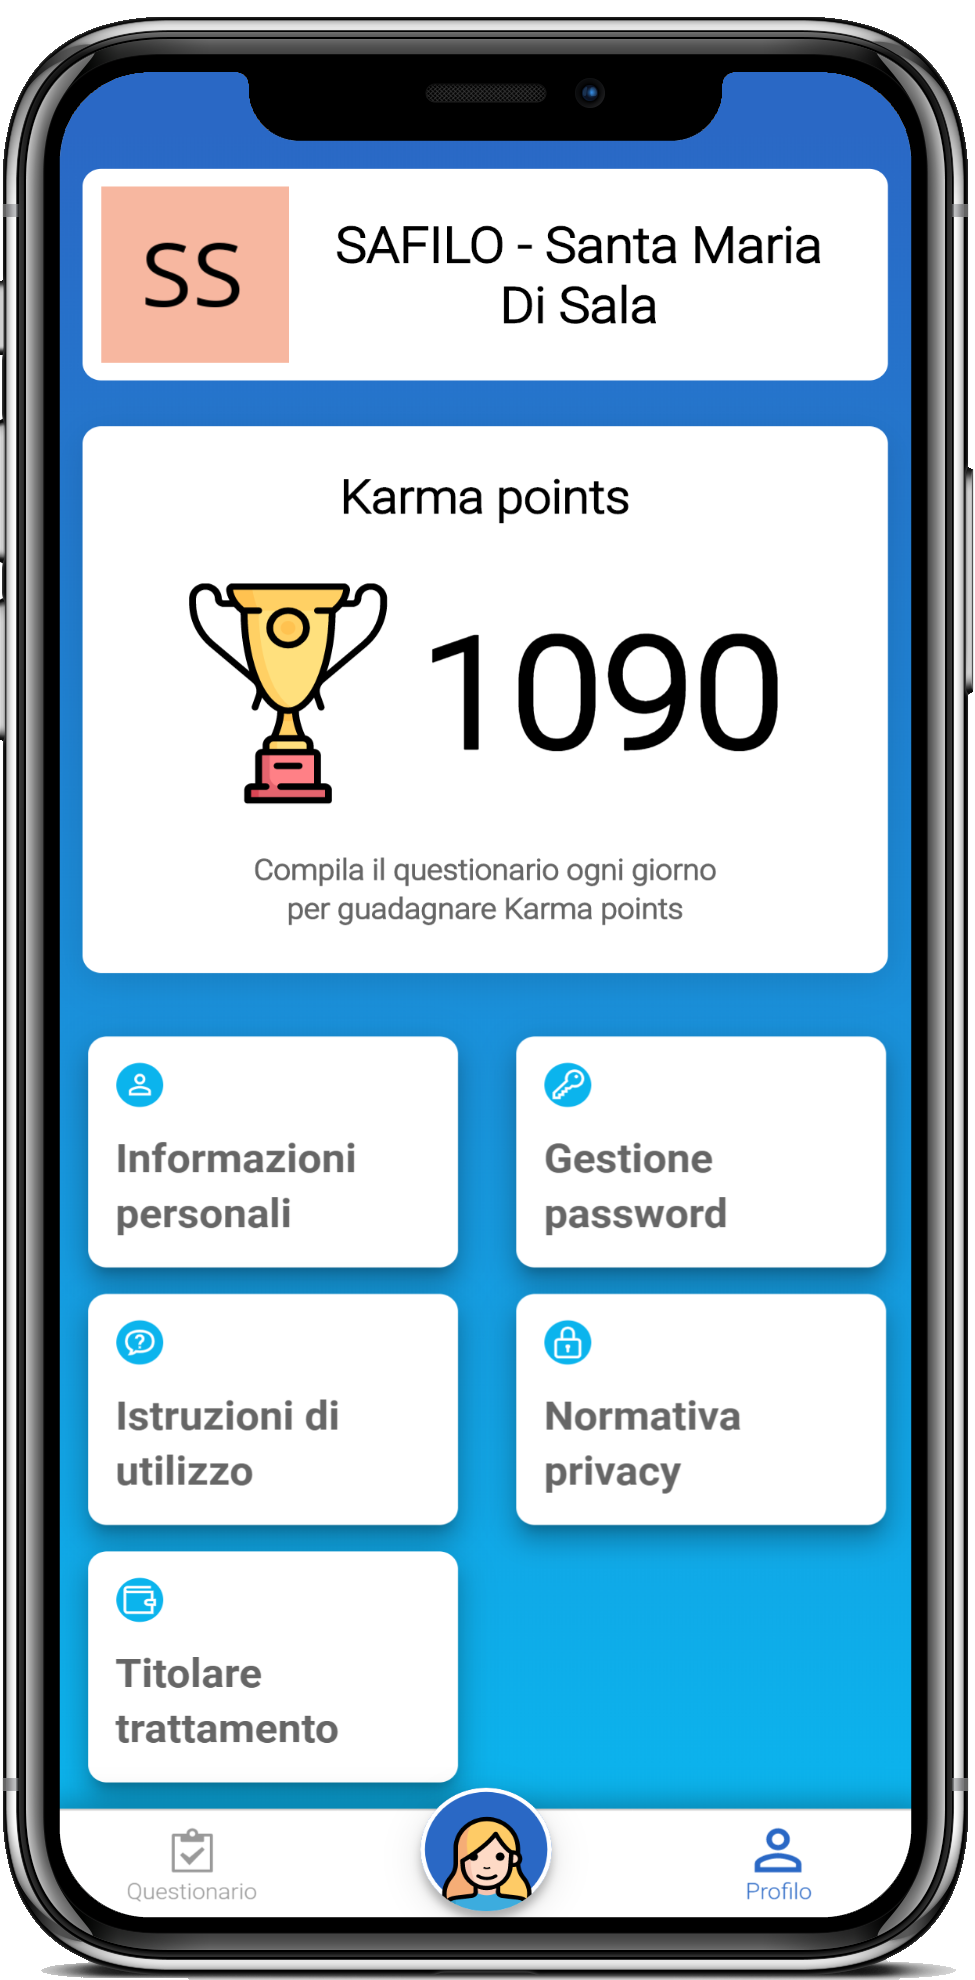
\includegraphics[scale=0.11]{profile.png}
			\caption{Sezione Profilo}\label{fig:profile}
			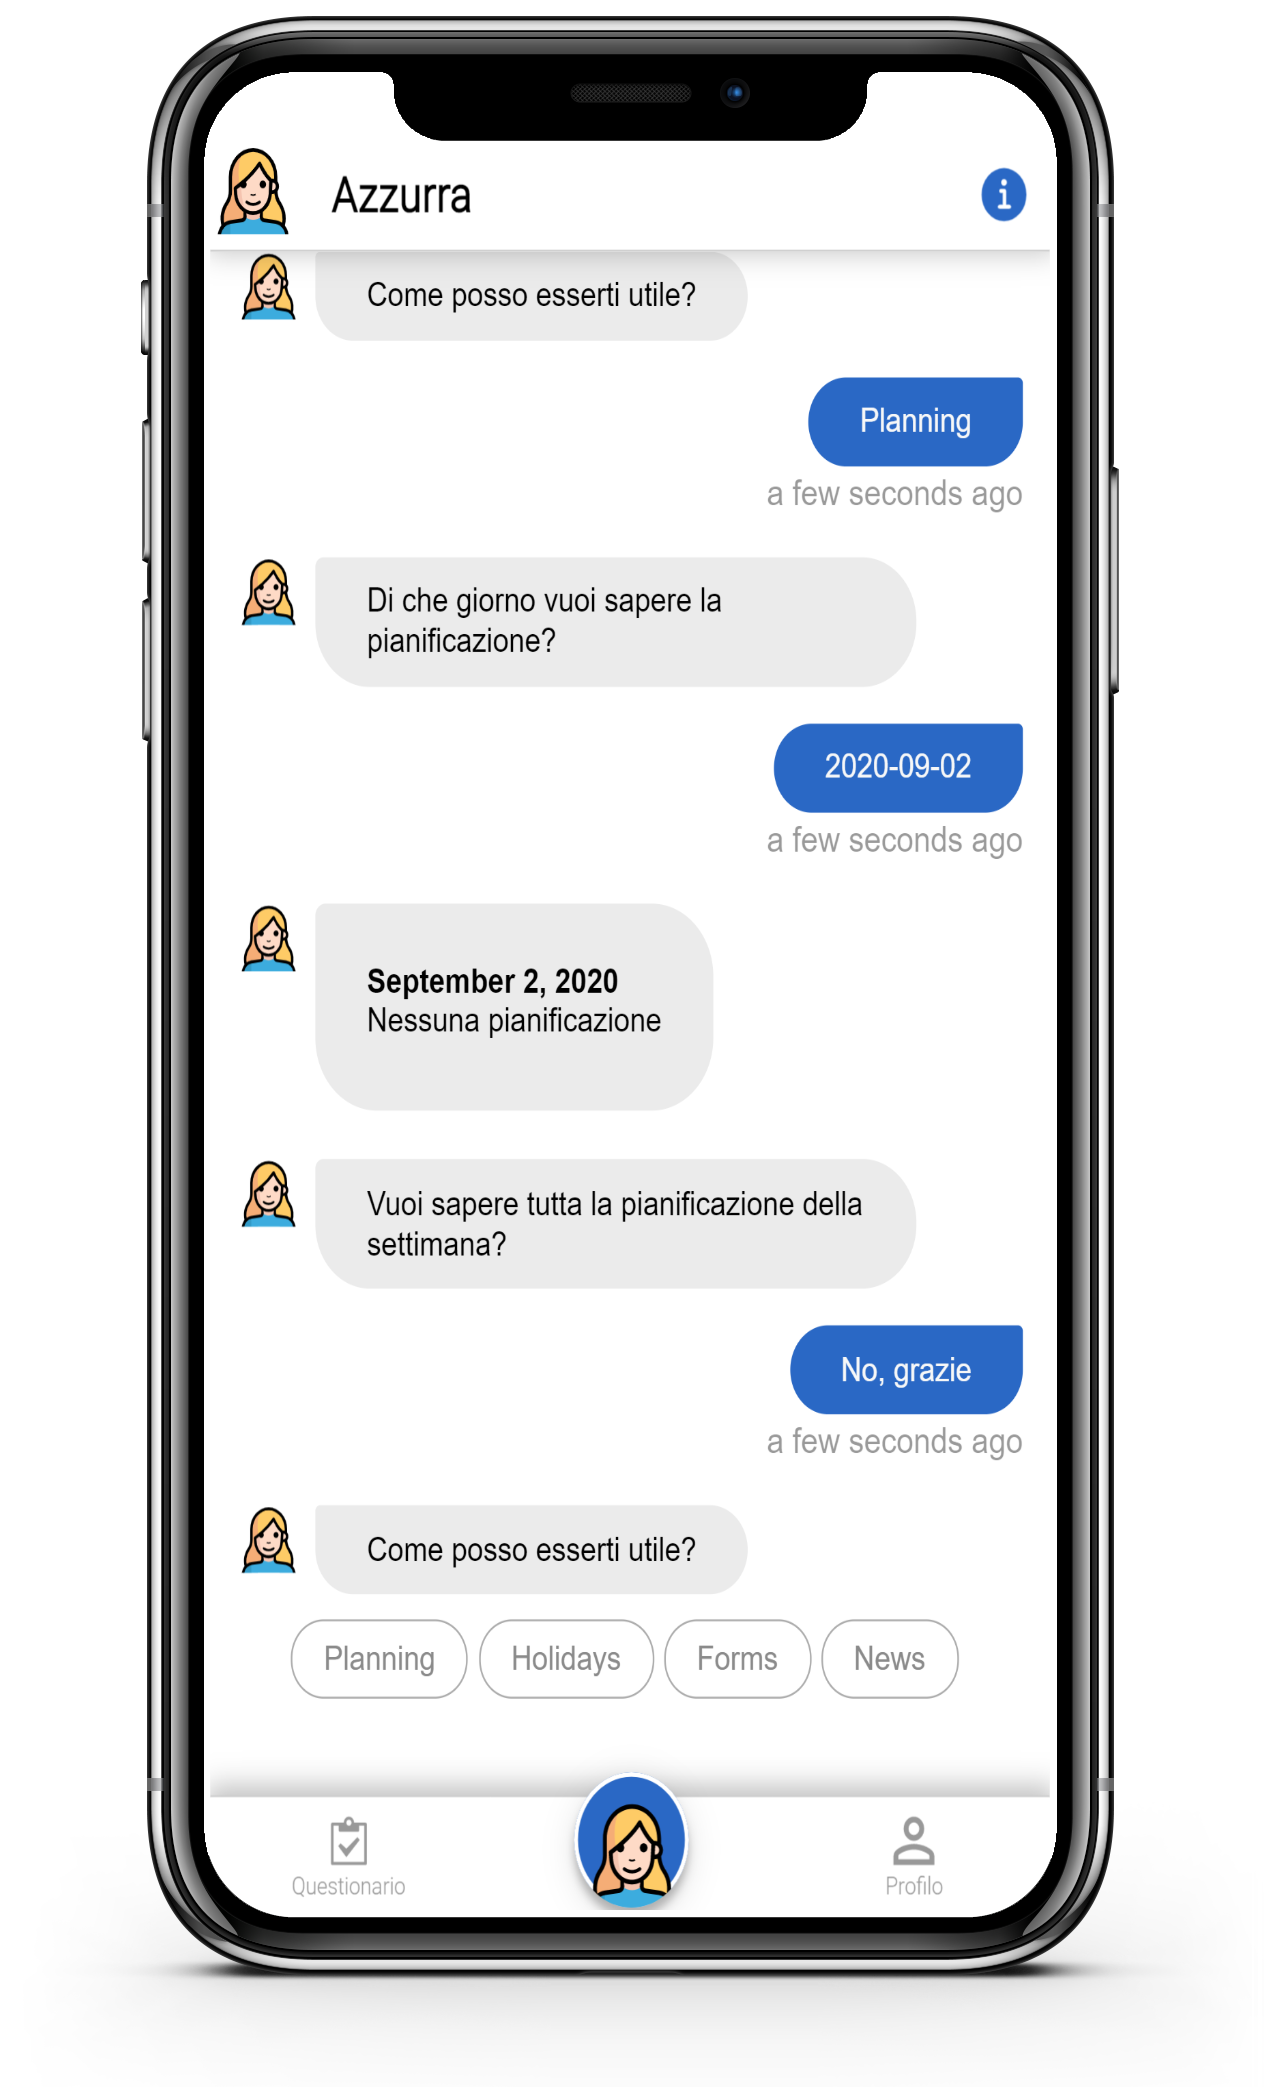
\includegraphics[scale=0.11]{chatAzzurra.png}
			\caption{Sezione Chat bot Azzurra}\label{fig:Azzurra}
		\end{center}
	\end{figure}\\
	Nella sezione Azzurra, è presente la chat bot con Azzurra che attraverso il proprio flow engine, riesce a comprendere i flussi conversazionali ricevuti in input da Azzurra.io. Grazie a ciò il bot Azzurra sa quali risposte e domande fare all'utente umano. Nel capitolo successivo verrà spiegato in modo dettagliato il funzionamento del Flow engine di Azzurra. Come detto precedentemente la comunicazione con Azzurra.io avviene attraverso websocket che permette di tenere aggiornati i flussi conversazionali ricevuti da Azzurra.io nel caso in cui subiscano modifiche.	
	
\end{trivlist}
\section{Operazioni}

\subsection{Creazione di una connessione attreverso websocket}

\subsection{Recupero dei flussi conversazionali}

\subsection{Gestione notifiche push}
